\documentclass{article}

\usepackage{amsmath}
\usepackage{fancyhdr}
\usepackage{graphicx}
\graphicspath{{}}

%% some colours
\usepackage{color}
\definecolor{deepblue}{rgb}{0,0,0.5}
\definecolor{deepred}{rgb}{0.6,0,0}
\definecolor{deepgreen}{rgb}{0,0.5,0}
\definecolor{backcolour}{rgb}{0.95,0.96,0.93}

%%%%%%%%%%%%%% CODE STUFF %%%%%%%%%%%%%%
%%%%%%%%%%%%%%%%%%%%%%%%%%%%%%%%%%%%%%%%
\usepackage{cprotect} % to be used in sol
\usepackage{listings} % for code display
% setting code style
\newcommand\pythonstyle{\lstset{
        language=Python,
        backgroundcolor=\color{backcolour},
		basicstyle=\footnotesize,
		otherkeywords={self},
		keywordstyle=\footnotesize\color{deepblue},
		emph={__init__},
		emphstyle=\footnotesize\color{deepred},
		stringstyle=\color{deepgreen},
		frame=single,
		showstringspaces=false  ,
		breaklines=true,
		numbers=left,
		numberstyle=\footnotesize,
		tabsize=4,
		breakatwhitespace=false
	}}

% Python environment
\lstnewenvironment{python}[1][]{
    \pythonstyle
    \lstset{#1}
}{}

% Python for external files
\newcommand\pythonexternal[2][]{{
    \pythonstyle
    \lstinputlisting[#1]{#2}
}}

% Python for inline
\newcommand\pythoninline[1]{{\pythonstyle\lstinline!#1!}}

%%%%%%%%%%%%%%%%%%%%%%%%%%%%%%%%%%%%%%%%
% setting the style for ex documents
\pagestyle{fancy}
\fancyhf{}
\fancyhead[L]{\thetitle}
\fancyhead[C]{}
\fancyhead[R]{\theauthor}
\renewcommand{\headrulewidth}{0.4pt} %obere Trennlinie
\fancyfoot[L]{Due: \thedate}
\fancyfoot[R]{\thepage} %Seitennummer
\renewcommand{\footrulewidth}{0.4pt}

% include solutions
\newcommand\sol[1]{{\large\textbf{\\Solution:}}#1}


\title{BPP Exercise 4 - Lists and Collections}
\author{A. Hain, M. Nipshagen}
\date{30.04.2018, 8:00}

\makeatletter
\let\thetitle\@title
\let\theauthor\@author
\let\thedate\@date
\makeatother

% Defining the Left Pointy Bracket and the Right Pointy Bracket, so they look nicer
\newcommand\lpb{\small{<}}
\newcommand\rpb{\small{>}}
% sublists are annoying
\newcommand\SubPoint[1]{
  \begin{itemize}
    \item #1
  \end{itemize}
  }
  
% do not include solutions
% \renewcommand\sol[1]{} \renewcommand\SubPoint[1]{}


\begin{document}

The deadline for this exercise sheet is \textbf{Monday, \thedate.}
%
%\section*{Introductory Words}
%In case we have some information that doesn't directly concern the current exercises.
%
\section{Vector Math}
We can model vectors with tuples and lists. Python however is not equipped with the tools to do vector math, but we can write the functions for this ourselves!\\
Write a script \texttt{vectors.py} which defines the following functions:
\begin{itemize}
  \item \texttt{add(x, y)}: Adds $x$ and $y$ such that the result follows $z_i = x_i + y_i$.
    \cprotect\sol{
\begin{python}
def add(x, y):
      """Adds up the vectors x and y"""
      return [x[i] + y[i] for i in range(len(x))]
\end{python}
    }
  \item \texttt{sub(x, y)}: Subtracts $y$ from $x$ such that the result follows $z_i = x_i - y_i$.
    \cprotect\sol{
\begin{python}
def sub(x, y):
    """returns the result of subtracting y from x"""
		return [x[i] - y[i] for i in range(len(x))]
\end{python}
    }
  \item \texttt{dot(x, y)}: Calculates the scalar (dot) product (or inner product) of $x$ and $y$. The dot product $\lpb x,y\rpb$ is defined as $\lpb x,y\rpb = \sum\limits_{i=1}^{N}x_iy_i$.
\cprotect\sol{\begin{python}
def dot(x, y):
    """Returns the inner product of the two vectors"""
		sum([x[i]y[i] for i in range(len(x))])
	\end{python}}
  \item \texttt{angle(x, y)}: Calculates the angle $\theta$ between the between $x$ and $y$. The angle can be found by using an alternative definition of the dot product: $\lpb x,y\rpb = \|x\|\|y\| \cos\theta$, which we can then solve for $\theta$ and we get $\theta = \arccos\dfrac{\lpb x,y\rpb}{\|x|\|y\|}$.\\
  \emph{Note:} $\|x\|$ where $x$ is a vector is called the vector norm and is calculated by $\sqrt{<x,x>}$. You can find the arccos function in the \texttt{math} package, which we previously used for pi. The function is called \texttt{acos}.
\cprotect\sol{\begin{python}
import math


def angle(x, y):
    """Returns the angle between the two vectors in radien"""
    divisor = math.sqrt(dot(x, x)) * math.sqrt(dot(y, y))
		return math.acos(dot(x, y) / divisor)
	\end{python}}
  \item \texttt{pdist(x, y, **kwargs)}: The distance between the two points $x$ and $y$. Your \textit{kwargs} should recognise the keywords \texttt{metric} and \texttt{p}. Your \texttt{metric} keyword should be able to take one of the values \texttt{'euclidean', 'minkowski', 'cityblock'}, and \texttt{p} can take any integer greater or equal than one. The distance is calculated depending on the metric and should default to \texttt{euclidean}. The distances are calculated as follows:
    \begin{itemize}
      \item \texttt{euclidean}: $d_{euclid} (x,y) = \sqrt[\uproot{2}2]{\sum\limits_{i=1}^N \|x_i-y_i\|^2}$.
      \item \texttt{minkowski}: $d_{minkowsky} (x,y) = \sqrt[\uproot{2}\texttt{p}]{\sum\limits_{i=1}^N \|x_i-y_i\|^\texttt{p}}$.
      \item \texttt{cityblock}: $d_{cityblock} (x,y) = \sum\limits_{i=1}^N \|x_i-y_i\|$\\
      (\emph{Note:} $\|x\|$ is the absolute value.)
    \end{itemize}
    See figure \ref{fig:metrics} for a nicer visualisation.\\
    Don't be afraid of this. It looks scary at first, but it is not beyond the scope of what you already learned.
\cprotect\sol{\begin{python}
import math


def pdist(x, y, **kwargs):
    """
    Calculates the distance between x and  y using the given metric.

    The default metric used for distance calculation is the euclidean metric. Other options are 'cityblock' and 'minkowski'. If using minkowski distance, the parameter p >= 1 can be supplied.
    """
    # check whether metric is given, and use euclidean as default
	metric = 'euclidean'
    if 'metric' in kwargs:
        metric = kwargs['metric']
        # if minkwoski is used, check if p is supplied, else use 2 (euclidean)
        if metric == 'minkowski':
            if 'p' in kwargs:
                p = kwargs['p']
            else:
                p = 2
    
    if metric == 'euclidean':
        squared = [abs(x[i] - y[i])**2 for i in range(len(x))]
        return math.sqrt(sum(squared))
    elif metric == 'cityblock':
        diff = [abs(x[i] - y[i]) for i in range(len(x))]
        return sum(diff)
    elif metric == 'minkowski':
        if p < 1:
            return None
        to_p = [abs(x[i] - y[i])**p for i in range(len(x))]
        return sum(to_p) ** (1/p)
    else:
        return None
\end{python}
}
  \item \textbf{BONUS:} \texttt{outer(x, y)}: calculates the outer product of two vectors. The outer product of two vectors is the tensor product of the two. For two vectors with size $n$ the outer product will yield a matrix of size $(n, n)$.
  The outer product is calculated as $C_{i_j} = x_iy_j$.
  \cprotect\sol{\begin{python}
def outer(x, y):
		"""Returns a list of lists representinx a matrix calculated from the two vectors, each list represents one row"""
    result = []
    for i in range(len(x)):
        row = []
        for j in range(len(y)):
          row.append(x[i] * y[j])
        result.append(row)
		return result
	\end{python}}
\end{itemize}
You can assume that all vectors have the same size. To verify your function works correctly you can test it with the following values:\\
$a = (1, 2, 3), b = (4, 5, 6), c = [0, 1, 0, 0, 1], d = [1.5, 2.5, 3.5, 4.5, 5.5]$\\
\begin{tabular}{|ll|}
  \hline
  Call & Result \\
  \hline
  \texttt{add(a,b)} & (5, 7, 9)\\
  \texttt{add(b,a)} & (5, 7, 9)\\
  \texttt{sub(a,b)} & (-3, -3, -3)\\
  \texttt{dot(c,d)} & 8.0\\
  \texttt{angle(a,b)} & approx. 0.23\\
  \texttt{pdist(a,b)} & approx. 5.20\\
  \texttt{pdst(a,b, metric='cityblock')} & 9\\
  \texttt{pdist(c,d, metric='minkowski', p=3)} & 6.14\\
  \texttt{outer(a,b)} & $\left[\begin{matrix} 4 & 5 & 6\\ 8 & 10 & 12\\ 12 & 15 & 18 \end{matrix}\right]$\\
  \hline
\end{tabular}
\begin{figure}
  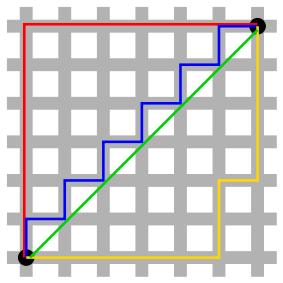
\includegraphics[scale=0.5]{metriken}
  \label{fig:metrics}
  \caption{Blue, red, and yellow are examples for the cityblock distance (it looks like following the streets of a grid city) and green is the euclidean distance.}
  \small{Taken from \url{https://en.wikipedia.org/wiki/Taxicab_geometry#/media/File:Manhattan_distance.svg}}
  
\end{figure}

\section{Which to What}
We will give you a few examples of datasets. Which collection type would you use to save this data in?\\
Please explain your answers.
\begin{itemize}
\item options a user can click on in a program menu
\SubPoint{\sol{List}}
  \item a country's name, population and capital
    \SubPoint{\sol{Tuple or Dict}}
  \item food ingredients
    \SubPoint{\sol{List}}
  \item data about a music album
    \SubPoint{\sol{Dict}}
  \item people who visit Basic Programming in Python or Scientific Programming in Python
    \SubPoint{\sol{Set}}
  \item IDs of upcoming orders in an online shop
    \SubPoint{\sol{List}}
  \item nicknames and account information in a forum (e-mail address, password, real name [optional], birth date [optional], ...)
    \SubPoint{\sol{Dict}}
\end{itemize}

\section{The Transform}
In the file \texttt{my\_collection.py} you will find two lists defined: \texttt{subjects} and \texttt{attributes}. The first list contains subject ids, wheras the second one contains attributes corresponding to the subject ids. So the subject at index 0 of \texttt{subjects} has the attribute at index 0 of \texttt{attributes} and the subject at index 9 has the attribute at index 9. You get the idea.\\
You may notice that each subject id appears multiple times. Your task now is to create a function to create one dictionary which uses the subject id as a key and a \textit{list} of attributes as the value.
\end{document}
